\documentclass[A4paper, 12pt]{amsart}

\usepackage{amsmath}
\usepackage{amsfonts}
\usepackage{amssymb}
\usepackage[]{hyperref}
%\usepackage[english]{babel}
\usepackage[utf8]{inputenc}
\usepackage[]{graphicx}
\usepackage{xcolor}
\usepackage{tikz}
\usepackage[margin=1.5cm]{geometry}

\linespread{1.5}

\title{Tutorium der Elektrodynamik}
\author{Alejandro Gallo}


\begin{document}

\maketitle
\tableofcontents

\section{Zylindrischer Kondensator}
Hier werden wir einige typische Beispiele
besprechen, die im Rahmen von der Kondensatorthematik
auftauchen.
Dafür werden wir den aus der Vorlesung bekannten Satz
%
\begin{equation}
  %Equation for gauss theorem
  \label{eq:gauss_theorem}
  \nabla ^{2} V(\mathbf{r}) = \rho / \epsilon_{0}
\end{equation}
%
brauchen.

In einem zylindrisch symmetrischen Problem, d.h., wo das Potential
$ V $ nur von $ r $ abhängt, ($ V(r, \phi, z) = V(r) $) gilt
%
\begin{equation}
  %Equation for laplacian in cylindrical coordinates
  \label{eq:laplacian_in_cylindrical_coordinates}
  \nabla ^{2} V(\mathbf{r}) =
  \frac{1}{r}
  \frac{\mathrm{d}}{\mathrm{d}r}
  r
  \frac{\mathrm{d}}{\mathrm{d}r}
  V(r)
  .
\end{equation}
%

\newpage
\subsection{Potential im Inneren einer einfachen zylindrischen Platte}

Wir betrachten einen Zylinder mit Radius $ R_{0} $ und einen
Zylinder als Integrationsvolumen $ G $.

\begin{center}
  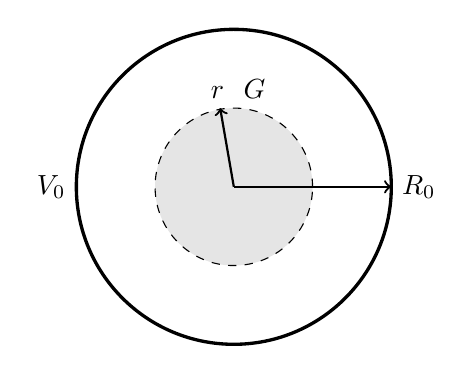
\begin{tikzpicture}
  \draw[very thick]
    (0,0) circle [radius=2cm]
    ++ (2cm,0) node (R0) [right] {$R_0$}
    (0,0) ++ (-2cm,0) node  [left] {$V_0$}
  ;
  \draw[dashed, fill=black!10]
    (0,0) circle [radius=1cm]
    ++ (0,1cm) node [above right] {$G$}
    node (G) [above left] {$r$}
  ;
  \draw[->, thick] (0,0) -- (R0);
  \draw[->, thick]
    (0,0) -- (G)
  ;
\end{tikzpicture}


\end{center}

Es wird nämlich eine Funktion $ V(r) $ gesucht, wo
$ 0 \leq r < R_{0} $.
Wir versuchen zuerst, Gleichung~\ref{eq:gauss_theorem} direkt
zu lösen.
Im $ G $ gibt es keine Ladung, also $ \rho =0 $ und folglich %
\begin{align*}
  \frac{1}{r}
  \frac{\mathrm{d}}{\mathrm{d}r}
  r
  \frac{\mathrm{d}}{\mathrm{d}r}
  V(r)
  =0
\end{align*}
%
woraus folgt dass
\begin{align*}
  r
  \frac{\mathrm{d}}{\mathrm{d}r}
  V(r)
  = A,
  \qquad \Rightarrow \qquad
  \frac{\mathrm{d}}{\mathrm{d}r}
  V(r)
  =
  \frac{A}{r}
\end{align*}
wobei $ A $ eine Konstante ist.
Wir können von einem beliebigen Ort $ r_{0} $ bis $ r $ integrieren, solange
$ r_{0} $ innerhalb des Zylinders bleibt,
%
\begin{align*}
  \int_{r_{0}}^{r}
    \frac{\mathrm{d}}{\mathrm{d}r}
    V(r')
  \mathrm{d} r' =
  V(r) - V(r_{0}) =
  \int_{r_{0}}^{r}
    \frac{A}{r'}
  \mathrm{d} r' =
  A \ln \frac{r}{r_{0}}
\end{align*}
%
woraus wir den allgemeinen Ausdruck für die Lösung bekommen,
%
\begin{equation}
  V(r) =
  A \ln \frac{r}{r_{0}}
  +
  B
  .
\end{equation}
%
Es ist bemerkenswert dass man zwei Bedingungen benötigt, um die
Integrationskonstanten $ A $ und $ B $ zu bestimmen.
Dies ist so da
Gleichung~\ref{eq:gauss_theorem} eine Differentialgleichung zweiter Ordnung
ist. Im allgemeinen finden wir aber dass
%
\[
  V(r_{0}) = B.
\]
%
In dem Sinne, wenn wir
$ r_{0} = R_{0}$ setzen können wir
\begin{equation}
  V(r) =
  A \ln \frac{r}{r_{0}}
  +
  V_{0}
\end{equation}
schreiben.
Wir haben aber nicht genügende Bedingungen um $ A $ zu bestimmen.
Das ist, wir können nicht \textit{Cauchy Randbedingungen} verwenden
weil wir nur eine Information zur Verfügung haben, nämlich dass
$ V(R_{0}) = V_{0} $.
Wir müssen dann erkunden wie die Ableitung der Funktion $ V $ (das heißt,
das elektrische Feld) aussieht. Wenn dies uns gelingt dann wird es uns
ermöglichen, Bedingungen für die erste Ableitung von $ V $ zu finden,
dementsprechend arbeiten wir hier mit \textit{Dirichlet Randbedingungen}.
Wir können das Volumen $ G $ dafür verwenden:
%
\begin{align*}
  0
  =
  \int_{G}
    \nabla \cdot \mathbf{E}
  \ \mathrm{d}^{3} x
  =
  \int_{\partial G}
    \mathbf{E} \cdot \mathrm{d}\mathbf{S}
  =
  E S
\end{align*}
%
und deswegen haben wir im Inneren $ \mathbf{E} = 0 $, $ V = V_{0} $.
Daraus folgt, dass $ A = 0 $ und somit haben wir die fehlende
Integrationskonstante $ A $ bestimmt, nämlich mittels \textit{Dirichlet
Randbedingungen}.

\subsection{Potential im Inneren eines einfachen zylindrischen Kondensators}

\begin{center}
  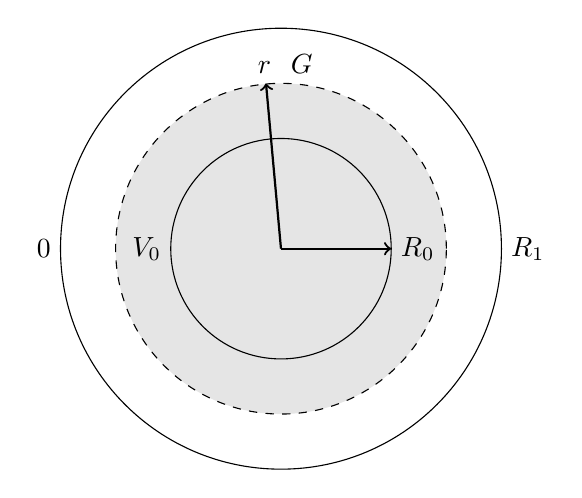
\begin{tikzpicture}[scale=0.7]
  \draw[dashed, fill=black!10]
    (0,0) circle [radius=3cm]
    ++ (0,3cm) node [above right] {$G$}
    node (G) [above left] {$r$}
  ;
  \draw[->, thick] (0,0) -- (G);
  \draw
    (0,0) circle [radius=2cm]
    ++ (2cm,0) node (R0) [right] {$R_0$}
    (0,0) ++ (-2cm,0) node  [left] {$V_0$}
  ;
  \draw[->, thick] (0,0) -- (R0);
  \draw
    (0,0) circle [radius=4cm]
    ++ (4cm,0) node (R1) [right] {$R_1$}
    (0,0) ++ (-4cm,0) node  [left] {$0$}
  ;
\end{tikzpicture}


\end{center}

Hier die Lösung von vorhin gilt noch da im Abstand
$ r $ das Problem noch zylindrisch symmetrisch bleibt.
Deswegen wissen wir dass im Zwischenraum das Potential $ V $
\begin{equation}
  V(r) =
  A \ln \frac{r}{R_{1}}
  +
  V(R_{1})
\end{equation}
ist.
In diesem Fall können wir aber $ A $ bestimmen da
\textit{Dirichlet Randbedingungen}
herrschen, d.h., wir haben zwei Punkte für die Randbedingungen.
Diese Randbedingungen lauten
%
\begin{equation*}
  \left\{
    \begin{matrix}
      V(R_{0}) & = & V_{0} \\
      V(R_{1}) & = & 0 \\
    \end{matrix}
  \right.
\end{equation*}
%
wie aus dem Bild abzulesen ist.
Die $ R_{1} $ Randbedingung ist schon von unserem Potential $ V(r) $ erfüllt,
für die zweite müssen wir folgendes schreiben
%
\begin{equation*}
  V(R_{0}) = V_{0} =
  A \ln \frac{R_{0}}{R_{1}}
  +
  0,
  \qquad \Rightarrow \qquad
  A =
  -
  \frac{V_{0}}{\ln \frac{R_{1}}{R_{0}}}
  =
  \frac{V_{0}}{\ln \frac{R_{0}}{R_{1}}}
\end{equation*}
%
und deswegen wenn $ R_{0} \leq r \leq R_{1} $
\begin{equation*}
  V(r) =
  V_{0}
  \frac{\ln \frac{r}{R_{1}}}{\ln \frac{R_{0}}{R_{1}}}
\end{equation*}
and
\begin{equation*}
  E(r) =
  - \frac{\mathrm{d}V}{\mathrm{d}r}(r)
  =
  \frac{V_{0}}{\ln \frac{R_{1}}{R_{0}}}
  \frac{1}{r}
\end{equation*}

\subsection{Kapazität eines zylindrischen Kondensators}

Die Kapazität eines Kondensators ist durch den Ausdruck
%
\begin{equation*}
  C = \frac{Q}{V}
\end{equation*}
%
definiert, wobei $ Q $ der Betrag der Ladung im Kondensator ist.
Wir können die Ladung mittels folgender Gleichung ausrechnen
%
\begin{equation*}
  Q =
  \int_{V}
    \rho (\mathbf{r})
  \ \mathrm{d}^{3}x
  .
\end{equation*}
%
Wir müssen das Volumen $ V $ bestimmen, und man kann sich überzeugen,
dass wir über dem grauen Bereich in der darunterliegenden Abbildung
integrieren soll.
\begin{center}
  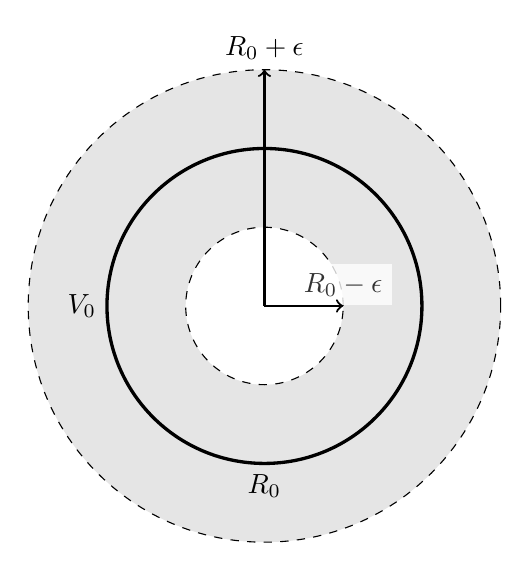
\begin{tikzpicture}[scale=1]
  \def\radiusZero{2cm}
  \def\eps{1cm}
  \draw[dashed, fill=black!10]
    (0,0) circle [radius=\radiusZero+\eps]
    ++ (0,\radiusZero+\eps) node (GPlus) [above] {$R_{0} + \epsilon$}
  ;
  \draw[dashed, fill=white]
    (0,0) circle [radius=\radiusZero-\eps]
    ++ (\radiusZero-\eps,0) node (GMinus) [right] {}
    node [above, rotate=-0, fill=white, opacity=0.8] {$R_{0} - \epsilon$}
  ;
  \draw[->, thick] (0,0) -- (GPlus);
  \draw[->, thick] (0,0) -- (GMinus);
  \draw[very thick]
    (0,0) circle [radius=\radiusZero]
    ++ (0,-\radiusZero) node (R0) [below] {$R_0$}
    (0,0) ++ (-\radiusZero,0) node  [left] {$V_0$}
  ;
\end{tikzpicture}


\end{center}

Dabei soll man bemerken welche Form das Potential $ V $ und die Ableitungen
davon übernimmt. Hierunter sind die Hauptmerkmale skizziert
\begin{center}
  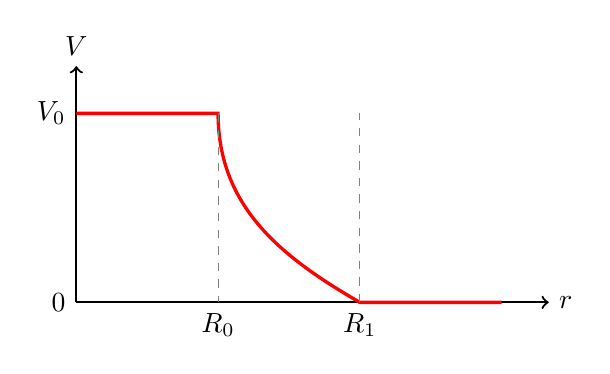
\begin{tikzpicture}
  \def\l{3cm}
  \def\lx{6cm}
  \def\V0{0.8*\l}
  \draw[->, thick]
    (0,0) coordinate (O)
    -- (0, \l) coordinate (y axis)
    node [above] {$V$}
  ;
  \draw[->, thick]
    (0,0) -- (\lx, 0) coordinate (x axis)
    node [right] {$r$}
  ;
  \draw[very thick, red]
    (0, \V0)
    node [left, black] {$V_0$}
    node at (O) [left, black] {$0$}
    --++ (0.3*\lx, 0) coordinate (r0)
    node at (r0 |- O) [below, black] {$R_0$}
    to[in=150, out=-90] (0.6*\lx, 0) coordinate(r1)
    node [below, black] {$R_1$}
    -- (0.9 * \lx, 0)
  ;
  \draw[dashed, black!50]
    (r0) -- (r0 |- O)
    (r1) -- (r1 |- r0)
  ;
\end{tikzpicture}
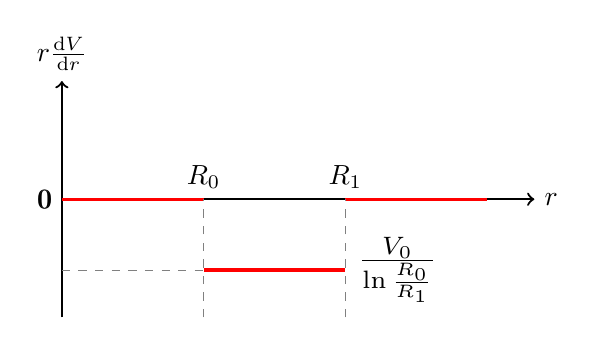
\begin{tikzpicture}
  \def\l{3cm}
  \def\lx{6cm}
  \draw (0,0.5*\l) coordinate (O) node [left] {$0$};
  \coordinate (Odown) at (0,0);
  \draw[->, thick]
    (Odown) -- (0, \l) coordinate (y axis)
    node [above] {$r\frac{\mathrm{d}V}{\mathrm{d}r}$}
  ;
  \draw[->, thick]
    (O) --++ (\lx, 0) coordinate (x axis)
    node [right] {$r$}
  ;
  \draw[very thick, red]
    (O)
    node at (O) [left, black] {$0$}
    --++ (0.3*\lx, 0) coordinate (r0)
    node at (r0 |- O) [above, black] {$R_0$}
  ;
  \draw[very thick, red]
    (r0) ++ (0, -0.3*\l)
    --++ (0.3*\lx, 0) coordinate(r1)
    node at (r1 |- O) [above, black] {$R_1$}
    (r1 |- O) --+ (0.3 * \lx, 0)
  ;
  \draw[dashed, black!50]
    (r0 |- Odown) -- (r0 |- O)
    (r1 |- Odown) -- (r1 |- r0)
    (r1 -| O)
    node at (r1)
      [right, black, scale=1.3] {$\frac{V_0}{\ln \frac{R_{0}}{R_{1}}}$}
    --++ (0.3*\lx, 0)
  ;
\end{tikzpicture}
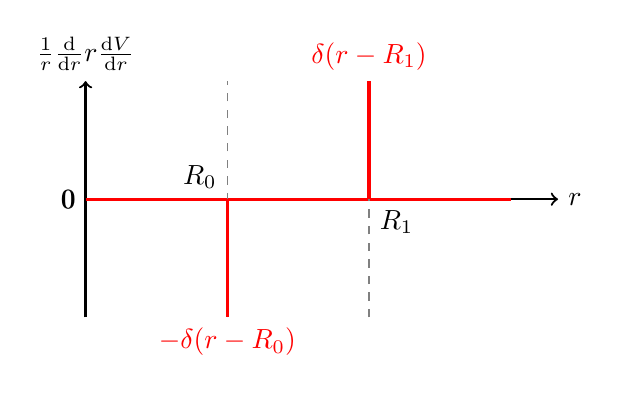
\begin{tikzpicture}
  \def\l{3cm}
  \def\lx{6cm}
  \draw (0,0.5*\l) coordinate (O) node [left] {$0$};
  \coordinate (Odown) at (0,0);
  \draw[->, thick]
    (Odown) -- (0, \l) coordinate (y axis)
    node [above]
      {$\frac{1}{r}\frac{\mathrm{d}}{\mathrm{d}r}r\frac{\mathrm{d}V}{\mathrm{d}r}$}
  ;
  \draw[->, thick]
    (O) --++ (\lx, 0) coordinate (x axis)
    node [right] {$r$}
  ;
  \draw[very thick, red]
    (O)
    node at (O) [left, black] {$0$}
    --++ (0.3*\lx, 0) coordinate (r0)
    node at (r0 |- O) [above left, black] {$R_0$}
  ;
  \draw[very thick, red]
    (r0) ++ (0, -0.0*\l)
    --++ (0.3*\lx, 0) coordinate(r1)
    node at (r1 |- O) [below right, black] {$R_1$}
    (r1 |- O) --+ (0.3 * \lx, 0)
  ;
  \draw[dashed, black!50]
    (r0 |- Odown) -- (r0 |- y axis)
    (r1 |- Odown) -- (r1 |- r0)
  ;
  \draw[very thick, red]
    (r0) -- (r0 |- Odown)
    node [below] {$-\delta(r - R_{0})$}
    (r1) -- (y axis -| r1)
    node [above] {$\delta(r - R_{1})$}
  ;
\end{tikzpicture}


\end{center}

\end{document}
